\begin{figure*}[tb]
  \centering
  \subfloat[\label{nonrandom}Linespoints]{
    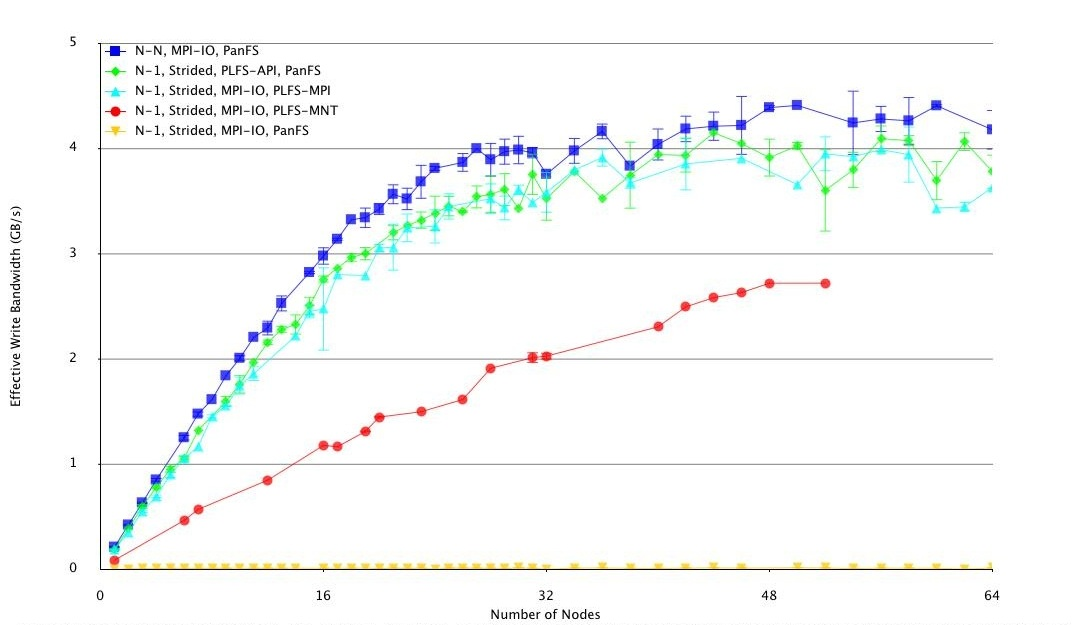
\includegraphics[width=0.3\textwidth,height=\figheight]{dbvizGraphsAndConfigs/allPoints.jpg}
  }
  \subfloat[\label{random}XY-scatter]{
    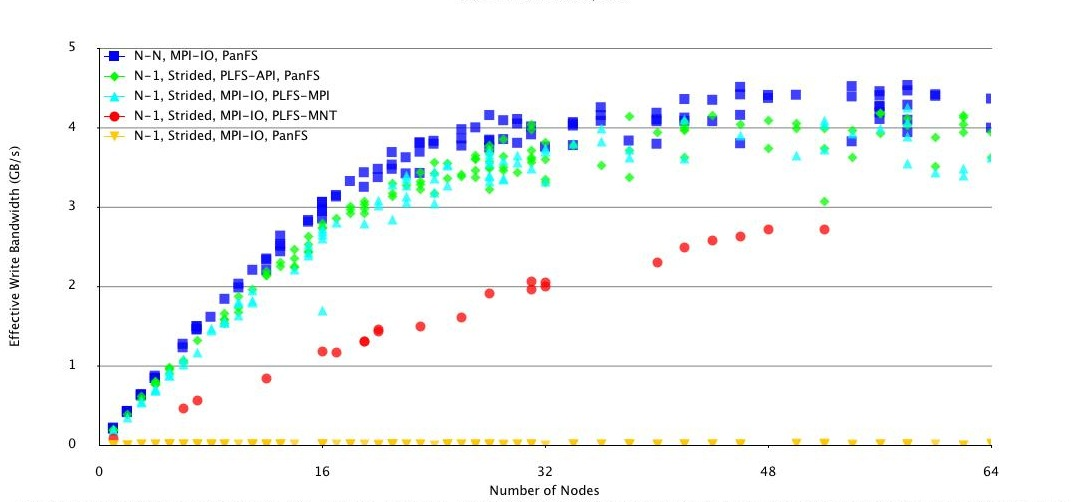
\includegraphics[width=0.3\textwidth,height=\figheight]{dbvizGraphsAndConfigs/allPointsAllScatter.jpg}
  }
  \subfloat[\label{random-full}Bars]{
    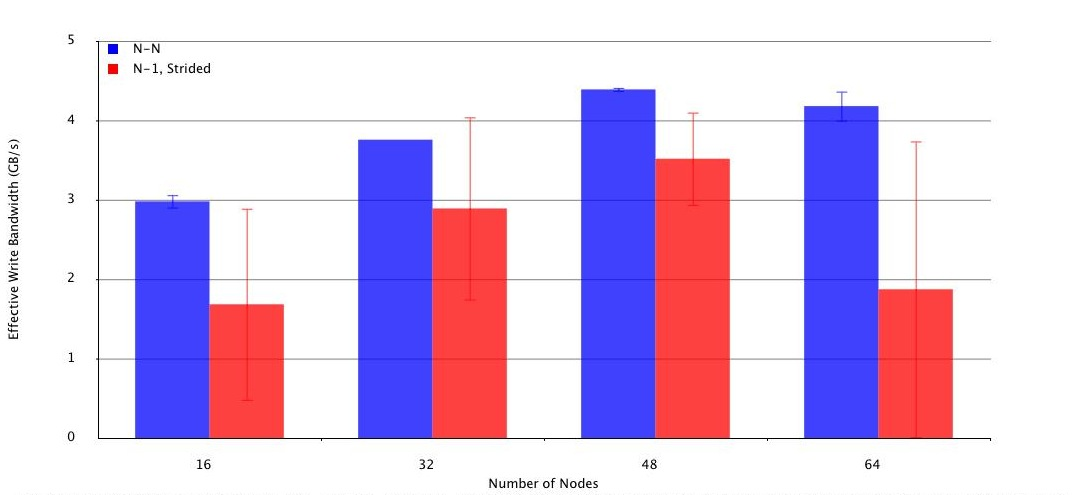
\includegraphics[width=0.3\textwidth,height=\figheight]{dbvizGraphsAndConfigs/allPointsBarGraph.jpg}
  }
  \mycaption{fig-dbviz}{Visualization Flexibility.}{
After \name\ populates a database with \kv\ pairs collected by transducers,
\dbviz\ allows interactive exploration of that data.  These figures 
show typical visualizations where a filter has been applied to the database,
and a visualization using the resulting rows is displayed.  One line (or bar) is
produced for each set of parameters that the user wishes to compare as a
function of specified values for both axes. The axes values can be a single
field or they can be arbitrarily complex combinations of multiple fields and
constants (\eg\ to show a bandwidth in GB/s, the user might specify that the
\yaxis\ should be a field dividing the number of bytes by a time and then 
dividing that again by a gigabyte).  The figure on the left shows an aggregation of
multiple points into mean values with standard deviations.  In the middle is
the same data in an xy-scatter plot; the scatter plot is useful because it allows
the user to easily identify outlying data.  The interactivity is vital here
as a user can click on an outlying data point and \dbviz\ will transparently
query the database and display a table of all \kv\ pairs for that outlier.
Finally, \dbviz\ can produce bar-graphs as well as in the figure on the right.
}
\end{figure*}

